\documentclass[12pt]{article}
% Свежая версия шаблона здесь <https://www.overleaf.com/read/sqvxbnhgxxdm>


\usepackage{fontspec}
\usepackage{polyglossia}
\usepackage{geometry}
\usepackage{graphicx}
\usepackage[final]{pdfpages}
\usepackage{amsmath,amsthm,amssymb,unicode-math}
\usepackage{wrapfig,multicol,tabularx,booktabs}
\usepackage[colorlinks=true, allcolors=blue]{hyperref}
\usepackage{xcolor}
%\usepackage{slashbox} %% разделение ячеек таблиц
%\usepackage{minted} %% листинги
%\usepackage{ulem} %% зачеркивание текста


\setmainlanguage{russian}
\setotherlanguage{english}
\setkeys{russian}{babelshorthands=true}

\defaultfontfeatures{Ligatures=TeX}
\setmainfont{CMU Serif Roman}
%\setmathfont{STIX Two Math}

\newfontfamily{\cyrillicfont}{CMU Serif Roman}
\newfontfamily{\cyrillicfontrm}{CMU Serif Roman}
\newfontfamily{\cyrillicfonttt}{Courier New}
\newfontfamily{\cyrillicfontsf}{CMU Serif Roman}
\newcommand{\const}{\mathrm{const}}

%\renewcommand{\thefigure}{\thesection.\arabic{figure}}
%\renewcommand{\thetable}{\thesection.\arabic{table}}
%\numberwithin{equation}{section}
\everymath{\displaystyle}
\graphicspath{{./img/}}
\renewcommand{\qedsymbol}{$\blacksquare$}
\theoremstyle{definition}
\newtheorem{definition}{Опр.}[]
\theoremstyle{remark}
\newtheorem{statement}{Утв.}[]
\theoremstyle{plain}
\newtheorem{theorem}{Теор.}[]
\newtheorem{axiom}{Аксиома}[]
\theoremstyle{definition}
\newtheorem{example}{Пример}[]
\addto\captionsrussian{
  \renewcommand{\figurename}{Рис.}
  \renewcommand{\tablename}{Табл.}
  \renewcommand{\proofname}{$\square$}
}

%% Дима
% Общее
\newcommand{\eps}{\varepsilon}
\renewcommand{\phi}{\varphi} % не работает
\renewcommand{\le}{\leqslant}
\renewcommand{\ge}{\geqslant}
% Для МСС
\newcommand{\e}{\bar{\vec{\mathrm{e}}}}
\newcommand{\zero}[1]{\stackrel{\raisebox{-2mm}{$\circ$}}{#1}}
% Для теорвера
\DeclareMathOperator{\mean}{M}
\DeclareMathOperator{\disp}{D}
\DeclareMathOperator{\cov}{cov}


\newcounter{QuestionID}
\newcommand{\supersection}[1]{
	\stepcounter{QuestionID}
	\section*{\arabic{QuestionID}. #1}
	\addcontentsline{toc}{section}{\arabic{QuestionID}. #1}
}


\begin{document}
    \supersection{Изображения как структура данных. Базовые операции над изображением. Свертка изображения}
        % Изображения как структура данных. Базовые операции над изображением. Свертка изображения


    \supersection{Морфологические операции. Эрозия, дилатация, замыкание и размыкание: что это и для чего могут быть использованы.}
        % Морфологические операции. Эрозия, дилатация, замыкание и размыкание: что это и для чего могут быть использованы.

\begin{definition}{Морфологическая операция}
    Пусть дано изображение $I$ в оттенках серого и некоторый структурный элемент $S$ -- небольшое черно-белое изображение, на котором выделена некоторая начальная точка (как правило, в центре изображения). Тогда под \textbf{морфологической операцией} понимается преобразование $I$ в выходное изображение $B$ такого же размера, где значение каждой точки $B_{ij}$ определяется по следующему правилу:
    \begin{enumerate}
    \item
        Структурный элемент совмещается с исходным изображением так, чтобы точка $I_{ij}$ совпала с начальной точкой $S$;
    \item
        Из исходного изображения выделяется набор точек, на которые накладываются белые точки структурного элемента;
    \item
        $B_{ij}$ определяется как некоторая заданная функция от значений выделенного набора точек (например, среднее, максимум/минимум)
    \end{enumerate}
\end{definition}

Выделяют следующие стандартные операции:

\paragraph{Эрозия.}

В случае эрозии заданная функция -- это минимум, поэтому эта операция также называется <<оконным минимумом>>. Эта операция полезна для удаления небольших объектов, в том числе шумов (в предположении, что объекты светлее фона), однако она затирает части объектов вблизи границы. Обозначение: $B = I \ominus S$.

\paragraph{Дилатация.}

Заданная функция -- максимум. В случае, если исходное изображение -- бинарное, эта операция эквивалентна смазу, при котором в качестве point spread function используется $S$. Обозначение: $B = I \oplus S$.

Взятие разности $I - \left( I \oplus S \right)$ может использоваться для выделения на изображении границ.

\paragraph{Замыкание (closing).}

Замыкание -- операция, которая задается как комбинация дилатации и эрозии (в таком порядке): $B = (I \oplus S) \ominus S$.

\paragraph{Размыкание (opening).}

Размыкание -- операция, которая задается как комбинация эрозии и дилатации (в таком порядке): $B = (I \ominus S) \oplus S$. Эта операция используется для выделения темного фона: сначала при помощи эрозии удаляются шумы и маленькие объекты, а затем при помощи дилатации восстанавливаются удаленные границы. При помощи вычитания размыкания из исходного изображения можно получить объекты, очищенные от фона. Это полезно, например, для выделения текста на изображении с неравномерным освещением, что можно видеть на изображении \ref{opening_demo}.

\begin{figure}[!h]
    \centering
    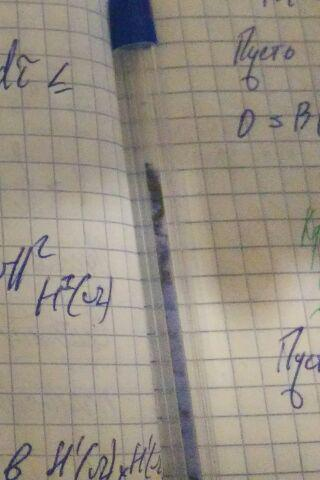
\includegraphics[width=0.3\linewidth]{2_orig}
    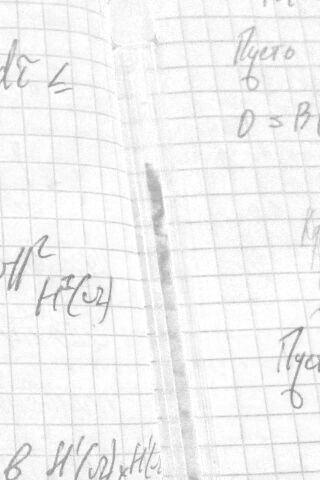
\includegraphics[width=0.3\linewidth]{2_diff}
    \caption{Исходное изображение (слева) и разность между исходным изображением и размыканием (справа).}
    \label{opening_demo}
\end{figure}


    \supersection{Фильтр границ Канни, для чего используется, какие параметры за что отвечают.}
        % Фильтр границ Канни, для чего используется, какие параметры за что отвечают.

Фильтр границ Канни (Кэнни) -- алгоритм, который среди всех пикселей изображения в градациях серого выделяет множество пикселей, которые образуют границы между объектами. Содержит следующие шаги:
\begin{enumerate}
\item
    Сглаживание изображения с целью устранения шума. Сглаживание выполняется путем сворачивания изображения с гауссовым ядром фиксированного размера: $I = H(\sigma) * I_0$. Слишком маленькие значения $\sigma$ не смогут убрать шум, что приведет к множеству ложноположительных срабатываний, а слишком большие превратят все изображение в слабо меняющийся градиент и уничтожат все границы.
\item
    Вычисление градиента, то есть полей частных производных яркости по двум координатам. Как правило, используется разностная схема размера $3 \times 3$, то есть свертка с ядром оператора Собеля:
    \begin{gather*}
        D_x = \begin{pmatrix}
            1 & 0 & -1\\
            2 & 0 & -2\\
            1 & 0 & -1
        \end{pmatrix},
        \quad
        D_y = D_x^T;\\
        G_x = D_x * I, \quad G_y = D_y * I. \\
    \end{gather*}
    Однако этот шаг может быть объединен с предыдущим: для этого нужно сворачивать исходное изображение с дифференцированным гауссовым ядром, то есть с дискретными приближениями $\partial_x h(0, \sigma), \partial_y h(0, \sigma)$.
\item
    По полученным значениям вычисляется массив абсолютных значений градиента ($G = \sqrt{G_x^2 + G_y^2}$, поэлементно) и массив направлений. Все направления округляются до одного из основных: вертикаль, горизонталь или одна из двух диагоналей, при этом сторона (влево или вправо) значения не имеет.
\item
    Все пиксели помечаются как границы или как не-границы по следующим правилам в указанном порядке:
    \begin{enumerate}
    \item
        Если элемент не является локальным максимумом в направлении \textit{своего} градиента, то элемент отмечается как не-граница. Например, если округленное направление градиента в $I_{ij}$ -- вертикаль, то $G_{ij} \le G_{i-1,j} \wedge G_{ij} \le G_{i+1,j} \implies B_{ij} = 0$, где $B$ -- выходной булев массив того же размера, что и изображение.
    \item
        Если модуль градиента $G_{ij} < \theta_{\mathrm{low}}$, то $B_{ij} = 0$.
    \item
        Если $G_{ij} > \theta_{\mathrm{high}}$, то $B_{ij} = 1$.
    \item
        В противном случае, если пиксель является локальным максимумом, но его абсолютное значение лежит между двумя пороговыми значениями, то он считается границей, если хотя бы один из 8 соседних был определен как граница с использованием предыдущего правила.
    \end{enumerate}
    
    Параметры $\theta_{\mathrm{low}}, \theta_{\mathrm{high}}$ регулируют количество ошибок обоих родов, но придать им какой-либо физический смысл довольно сложно.
\end{enumerate}


    \supersection{Преобразование Радона. Дискретное преобразование Радона. Оценка сложности.}
        % Преобразование Радона. Дискретное преобразование Радона. Оценка сложности.

\begin{definition}{Преобразование Радона}
    Пусть $l_{\theta, s}$ -- прямая, направляющий вектор которой направлен под углом $\theta$ ($\theta = 0$ соответствует горизональной прямой) и удаленная от начала координат на расстояние $s$. Тогда преобразованием Радона функции $f(x, y)$ называется интеграл этой функции по параметризованной прямой:
    \begin{gather*}
        \left[ \mathcal{R}f \right](\theta, s) =
        \int_{l_{\theta, s}} f(x, y) dl =
        \int_{\mathbb{R}^2} f(x, y) \delta(x \cos \theta + y \sin \theta - s) dx dy =\\=
        \int_{\mathbb{R}} f(s\cos\theta + z\sin\theta, s\sin\theta - z\cos\theta) dz.
    \end{gather*}
\end{definition}

Рассмотрим теперь дискретную версию $f(x, y)$, заданную, например, как среднее по квадратной области:
\begin{equation*}
    \hat{f}(i, j) =
    \frac{1}{h^2} \int_{ih - \frac{h}{2}}^{ih + \frac{h}{2}} \int_{jh - \frac{h}{2}}^{jh + \frac{h}{2}} f(x, y) dy dx.
\end{equation*}

Для определения дискретного преобразования Радона также необходим некоторый алгоритм дискретизации прямой $\Omega\left( s, \alpha \right)$, возвращающий множество координат пикселей $\left\{ \left( i_k, j_k \right)_{k=1}^{m} \right\}$, приближающих непрерывную прямую с соответствующими параметрами.

Тогда \textbf{дискретное преобразование Радона} определяется следующим образом:
\begin{equation*}
    \left[ \hat{\mathcal{R}} \hat{f} \right](\alpha, s) = \sum_{(i,j) \in \Omega(\alpha, s)} \hat{f}\left( i, j \right).
\end{equation*}

Однако такое определение обладает проблемой, связанной с неравномерностью приближения длины прямой количеством пикселей. Например, вертикальная непрерывная прямая, проходящая через центр квадрата со стороной $N$ имеет длину пересечения $N$, а диагональная -- $N\sqrt{2}$. Но обе дискретные версии будут иметь в пересечении с квадратом $N$ пикселей.


Оценим сложность преобразования Радона наивным способом. В разумной параметризации прямых количество дискретных прямых, которые проходят через изображение, составляет $O(n^2)$. Нужно вычислить и сохранить для каждой из них сумму по содержащимся в ней пикселям, количество которых $O(n)$. Считая, что $\Omega$ также обладает не более чем линейной сложностью по $n$, получаем, что для вычисления сумм требуется $O(n^3)$ операций и $O(n^2)$ памяти.

В случае черно-белых (бинарных) преимущественно черных изображений возможно изменить алгоритм: достаточно перебрать все белые точки и для каждой из них прибавлять единицу к сумме по всем прямым, проходящим через эту точку. Таким образом сложность понижается до $O(Cn^2)$, где $C$ -- количество белых точек на изображении. Однако необходимо учесть, что для этой вариации требуется уметь находить прямые, проходящие через заданную точку не более чем за $O(n^2)$ операций, что может быть затруднительно для некоторых видов параметризации.

    \supersection{Виды параметризации прямых на изображении и их свойства. Повторное вычисление преобразования Хафа и связь этой процедуры с поиском точки схода.}
        % Виды параметризации прямых на изображении и их свойства. Повторное вычисление преобразования Хафа и связь этой процедуры с поиском точки схода.


    \supersection{Преобразование Хафа и быстрое преобразование Хафа. Описание работы алгоритмов и их вычислительных характеристик.}
        % Преобразование Хафа и быстрое преобразование Хафа. Описание работы алгоритмов и их вычислительных характеристик.

% Радон: прямые, не обязательно дискретные.
% Хаф: дискретные объекты, не обязательно прямые.
% Дискретный Радон == Хаф для прямых.

В общем случае преобразование Хафа ставит в соответствие каждому паттерну из заданного семейства сумму значений пикселей изображения, принадлежащих этому паттерну. В данном случае рассматривается преобразование Хафа для дискретных прямых на двумерном изображении, которое также может быть названо дискретным преобразованием Радона.

Быстрое преобразование Хафа -- это вариация алгоритма, позволяющая понизить сложность алгоритма с $\Theta(n^3)$ до $\Theta(n^2 \log n)$ за счет использования диадических паттернов для приближения прямых.

Диадические паттерны описывают преимущественно вертиальные прямые с наклоном вправо, то есть в каждой строке $i=\const$ содержат ровно один пиксель и $j(i)$ нестрого возрастает. Они задаются следующим образом:
\begin{enumerate}
\item
    Существует один паттерн высоты 1, состоящий из одного пикселя
\item
    Существует $2^n$ паттернов высоты $2^n$ (или порядка $n$), $n > 0$. Паттерн под номером $i$ (нумерация начинается с нуля) состоит из двух состыкованных по вертикали паттернов высоты $2^{n-1}$ под номером $\left\lfloor \frac{i}{2} \right\rfloor$.
    Если $i$ четно, то нижний пиксель верхнего паттерна располагается над верхним пикселем нижнего паттерна.
    Если $i$ нечетно, то верхний паттерн дополнительно сдвигается на один пиксель вправо.
\end{enumerate}

В силу построения диадические паттерны содержит множество пересечений. В частности, любой паттерн высоты больше 1 делит как верхнюю, так и нижнюю половину с другим паттерном той же высоты. Поэтому для вычисления сумм по всем $n^2$ паттернам некоторого порядка достаточно вычислить $n^2$ сумм по паттернам меньшего порядка, а не $2n^2$, как было бы для наивной реализации.

Рассмотрим алгоритм БПХ более подробно. Пусть имеется квадратное изображение со стороной $N = 2^n$. Изначальное изображение можно рассматривать как набор сумм по паттернам порядка $0$. Чтобы получить в том же изображении набор сумм по паттернам порядка $1$, проделаем следующую операцию:
\begin{itemize}
\item
    Разделим изображение на $2^{n-0-1}$ групп, каждая из которых содержит $2^{0+1}$ последовательных строк.
\item
    Каждую группу разделим на верхнюю и нижнюю половины. Затем во все строки группы с номером $2i+r$ нужно записать поэлементную сумму $i$-х строк верхней и нижней половины, сместив строку из верхней половины вправо на $i+r$ элементов, где $i$ меняется от $0$ до $2^{0}$ невключительно (то есть, на начальной итерации $i=0$), а $r \in \{0, 1\}$ -- остаток от деления на 2.
\item
    В силу определения диадических паттернов, после предыдущего шага в $i$-й строке каждый группы записаны суммы по диадическим паттернам $1$ порядка с номером $i$, причем все они начинаются с различных элементов нижней строки группы.
\end{itemize}

Так как полученное в конце условие очень похоже на изначальное (набор сумм по паттернам порядка $1$), то неудивительно, что продолжная аналогичную операцию с соответственно увеличивающимися размерами групп после $n$ шагов мы получим массив, содержащий суммы по паттернам высоты $2^n = N$, начинающимся с $0$ строки изображения. Это и есть суммы по диадическим прямым определенного наклона. Для получения суммы по всем прямым, проходящим через изображение, следует воспользоваться БПХ для транспонированных/отраженных/... копий изображения и объединить полученные результаты.

Оценим сложность алгоритма быстрого преобразования Хафа. На каждой итерации значения каждого пикселя обновляются как сумма двух значений. При этом выполняется ровно $n$ итераций. Следовательно, итоговая сложность составляет $\Theta(N^2 \cdot n) = \Theta(N^2 \log N)$, где $N$ -- сторона изображения.

    \supersection{Трехмерное быстрое преобразование Хафа для плоскостей. Параметризация, описание работы, вычислительная сложность.}
        % Трехмерное быстрое преобразование Хафа для плоскостей. Параметризация, описание работы, вычислительная сложность.


    \supersection{Трехмерное быстрое преобразование Хафа для прямых. Параметризация, описание работы, вычислительная сложность.}
        % Трехмерное быстрое преобразование Хафа для прямых. Параметризация, описание работы, вычислительная сложность.

Трехемерное быстрое преобразование Хафа для прямых позволяет вычислять сумму по дискретным прямым в изображении размера $N \times N \times N$ вокселей. Рассматриваемые прямые -- преимущественно ориентированные вдоль оси $z$. Прямая параметризуется 4 параметрами и проходит через следующие воксели на верхней и нижней гранях куба:
\begin{equation*}
    (s_1, s_2, 0), \quad
    (s_1 + t_1, s_2 + t_2, N-1).
\end{equation*}

При этом считается, что все параметры могут меняться от $0$ до $N-1$. Заметим, что проекции прямой на плоскости $Oxz, Oyz$ представляют собой плоские диадические паттерны (в основном потому что именно так определяется трехмерная диадическая прямая).

Следовательно, для начала необходимо преобразовать изображение в четырехмерное. Исходное изображение располагается в пространстве с нулевой координатой по 4 измерению, все остальные пространства заполняются нулевыми значениями.
По аналогии с двумерным преобразованием, основная стратегия состоит в получении на каждом шаге отдельных <<слоев>>, значения в каждом из которых описывают суммы по всем возможным паттернам данной высоты $2^k$, начинающихся с низа данного слоя.
Но если в двумерном случае каждая группа должна была иметь размер $2^k \times N$, то для данного случая потребуются группы $N \times N \times 2^k \times 2^k$.
При этом первые две координаты практически не меняют своего смысла -- они соответствуют $s_1, s_2$, то есть описывают, в какой точке $x, y$ слоя \texttt{group[:, :, 0, 0]} (или, что то же самое, \texttt{image[:, :, 2**k * groupid, 0]}) начинается паттерн, описываемый вокселем. Третья координата $z$ -- это ось, вдоль которой распределяются и объединяются попарно группы. Четвертое измерение необходимо, чтобы было куда записывать получающиеся значения; при этом на $k$-й итерации используются только первые $2^k$ пространств, а остальные заведомо заполнены нулевыми значениями.

На каждом шаге две соседние группы объединяются в одну, и в двумерный срез с координатами \texttt{group[:, :, 2*i1+r1, 2*i2+r2]} записывается поэлементная сумма \texttt{group[:, :, i1, i2]} и \texttt{group[:, :, 2**k+i1, 2**k+i2]}, причем второй массив предварительно сдвигается на $(i_1+r_1, i_2+r_2)$ элементов по последним координатам. Например, после первой итерации группы будут иметь размер $N \times N \times 2 \times 2$, причем две последние координаты описывают тип паттерна (вертикальный, диагональный по одной координате, диагональный по другой координате или диагональный по обеим координатам).

На каждой итерации обрабатывается $\frac{N}{2^{k+1}}$ групп ($k=0, 1, \dots, \log_2 N - 1$). В каждой группе для всех значений $i_1, i_2, r_1, r_2$, то есть $2^{k} \cdot 2^{k} \cdot 2 \cdot 2 = 2^{2k+2}$ раз суммируются двумерные массивы из $N^2$ элементов. Таким образом, сложность алгоритма составляет
\begin{equation}
\label{complexity-fht-3d-lines}
    \Theta\left( \sum_{k=1}^{\log_2 N - 1} \frac{N}{2^{k+1}} \cdot 2^{2k+2} N^2 \right) =
    \Theta\left( 2N^3 + 4N^3 + 8N^3 + \dots + N^4 \right) =
    \Theta\left( N^4 \right).
\end{equation}

Наивная реализация потребовала бы $O(N^5)$ операций. Можно сказать, что трехмерное БПХ для прямых вычисляет сумму по каждой прямой в среднем за константное время.


% Предста8ьте куб, стоящий на столе на одной грани.
% Аккуратно по8ерните его на 45 градусо8 так, чтобы он стоял на одном ребре.
% Теперь по8ернте его еще раз на 45 градусо8 так, чтобы он стоял на одной 8ершине.
% За д8а шага получился куб, стоящий на столе одной точкой.

% За три шага аналогичную операцию можно проделать с тессерактом.
% Для простоты можно пропустить пер8ые д8а шага, 8зя8 куб, стоящий на 8ершине и распространи8 его на некоторое расстояние 8глубь по чет8ертому изменению. Осталось по8ернуть тессеракт 8сего один раз.


    \supersection{История развития томографии. Строение томографа.}
        % История развития томографии. Строение томографа.


    \supersection{Взаимодействие рентгеновского излучения с веществом. Сведение зарегистрированных данных к виду преобразования Радона.}
        % Взаимодействие рентгеновского излучения с веществом. Сведение зарегистрированных данных к виду преобразования Радона.


    \supersection{Преобразование Радона. Синограмма.}
        % Преобразование Радона. Синограмма.

\begin{definition}{Преобразование Радона}
    Пусть $l_{\theta, s}$ -- прямая, направляющий вектор которой направлен под углом $\theta$ ($\theta = 0$ соответствует горизональной прямой) и удаленная от начала координат на расстояние $s$. Тогда преобразованием Радона функции $f(x, y)$ называется интеграл этой функции по параметризованной прямой:
    \begin{gather*}
        \left[ \mathcal{R}f \right](\theta, s) =
        \int_{l_{\theta, s}} f(x, y) dl =
        \int_{\mathbb{R}^2} f(x, y) \delta(x \cos \theta + y \sin \theta - s) dx dy =\\=
        \int_{\mathbb{R}} f(s\cos\theta + z\sin\theta, s\sin\theta - z\cos\theta) dz.
    \end{gather*}
\end{definition}

Каждая точка Радон-образа функции представляет собой ``сумму'' по прямой с определенными параметрами. Как правило, по обоим параметрам рассматривается равномерная дискретная сетка значений, где $\theta$ меняется от $0$ до $\pi$, $s$ -- от $0$ до некоторого максимального значения, соответствующего размеру сцены. Полученный массив значений называется синограммой, так как Радон-образом точечной функции является синусоида.

    \supersection{Теорема о центральном сечении.}
        % Теорема о центральном сечении.

Преобразование Фурье функций от одной и от двух переменных задаются следующими формулами:
\begin{gather}
\label{fourier1D}
    \hat{f}(\omega) = \int_{\mathbb{R}} f(t) e^{-2\pi i (\omega t)} dt,\\
\label{fourier2D}
    \hat{F}(u, v) = \int_{\mathbb{R}^2} f(x, y) e^{-2\pi i (xu + yv)} dx dy.
\end{gather}

Также введем сокращенное обозначение для преобразования Радона, считая $\theta$ фиксированным параметром, а $s$ -- переменной:
\begin{equation*}
    p_\theta(s) := \left[ \mathcal{R}f \right]\left( \theta, s \right).
\end{equation*}

\begin{theorem}{О центральном сечении.}
\label{fourier_slice_thm}
    Преобразование Фурье от $p_\theta(s)$ совпадает со значениями двумерного преобразования Фурье от $f(x, y)$ на некоторой прямой:
    \begin{equation*}
        \hat{p}_\theta(\omega) = F(\omega\cos\theta, \omega\sin\theta)
    \end{equation*}
\end{theorem}
\begin{proof}
    Преобразуем определение преобразований Фурье и Радона, используя основное свойство дельта-функции (а также $\delta(t) = \delta(-t)$):
    \begin{gather*}
        \hat{p}_\theta(\omega) =
        \int_{\mathbb{R}} p_\theta(s) e^{-2\pi i \omega s} ds =\\=
        \int_{\mathbb{R}^3} f(x, y) \cdot \delta(x\cos\theta + y\sin\theta - s) e^{-2\pi i \omega s} dx dy ds =
        \int_{\mathbb{R}^2} f(x, y) e^{-2\pi i \omega \left( x\cos\theta + y\sin\theta \right)} dx dy;\\
        F(u=\omega\cos\theta, v=\omega\sin\theta) =
        \left.\int_{\mathbb{R}^2} f(x, y) e^{-2\pi i \left( x u + y v \right)}\right|_{\substack{u=\omega\cos\theta\\v=\omega\sin\theta}} =
        \hat{p}_\theta(s).
    \end{gather*}
\end{proof}

Таким образом, прямая, вырезанная из двумерного Фурье-образа исходной функции, проходящая через начало координат, фактически описывает интегралы этой функции вдоль всех прямых, параллельных вырезанной. Получить их можно при помощи обратного к \eqref{fourier1D} преобразования.

    \supersection{Алгоритм обратного проецирования (BP).}
        % Алгоритм обратного проецирования (BP).


    \supersection{Алгоритм FBP.}
        % Алгоритм FBP.

Как было показано ранее, алгоритм обратного проецирования легко описать и реализовать, но он не является вполне точным с математической точки зрения, поскольку опускает якобиан $|\omega|$. В результате этого, как правило, восстановленное изображение получается размытым, значения, близкие к началу координат, завышены, а далекие от начала координат, наоборот, занижены. Причина этого в том, что после дискретизации с равномерной сеткой по $s$ и $\theta$ через пиксели, близкие к началу координат, проходит большее количество дискретных прямых.

Алгоритм \textbf{filtered backprojection} состоит в использовании вместо \eqref{backprojection} более правильной формулы, выведенной в \eqref{fbp_proof}:
\begin{equation}
\label{filtered_backprojection}
    \left[ \mathcal{B}_{f}(p_\theta(s)) \right](x, y) = \int_0^\pi \mathcal{F}^{-1}\left[ |\omega| \hat{p}_\theta(\omega) \right]\left( x\cos\theta + y\sin\theta \right) d\theta.
\end{equation}

С точки зрения реализации следует добавить в алгоритм обратного проецирования дополнительный шаг: для каждого угла $\theta_i$ заменить <<сырые>> значения синограммы $p_{\theta_i}(s)$ на $\mathcal{F}^{-1}\left[ |\omega| \hat{p}_{\theta_i}(\omega) \right](s)$. Множитель $|\omega|$ называется \textbf{Ramp filter}.

\begin{figure}[!h]
    \centering
    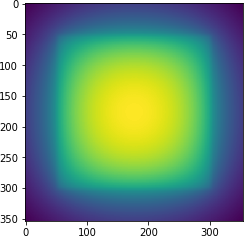
\includegraphics[width=0.3\linewidth]{backprojection_no_filter}
    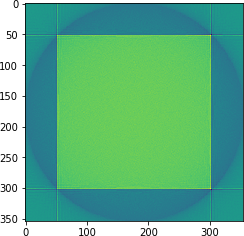
\includegraphics[width=0.3\linewidth]{backprojection_filtered}
    \caption{Восстановление белого квадрата из синограммы при помощи backprojection (слева) и filtered backprojection (справа).}
\end{figure}

    \supersection{Способ использования БПХ для определения наклона шрифта.}
        % Способ использования БПХ для определения наклона шрифта.

Быстрое преобразование Хафа может быть использовано для определения наклона шрифта. Рассмотрим следующее изображение:
\begin{figure}[!h]
    \centering
    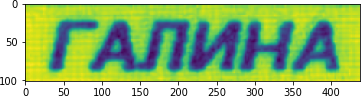
\includegraphics[width=0.7\linewidth]{15_1}
    \caption{Исходное изображение}
\end{figure}

Выделим на изображении границы путем вычитания из изображения его дилатации. Также здесь изображение было отражено относительно вертикальной оси, поскольку шрифт, очевидно, наклонен вправо, а стандартная версия быстрого преобразования Хафа работает с прямыми, наклоненными влево с точки стандартной системы координат изображения.
\begin{figure}[!h]
    \centering
    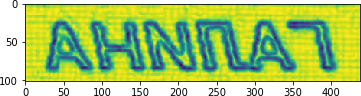
\includegraphics[width=0.7\linewidth]{15_2}
    \caption{Выделенные границы на изображении}
\end{figure}

Применим к полученному изображению БПХ:
\begin{figure}[!h]
    \centering
    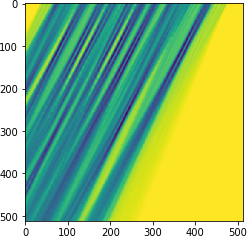
\includegraphics[width=0.35\linewidth]{15_3}
    \caption{Результат применения БПХ к изображению}
\end{figure}

В полученном массиве каждая точка описывает сумму значений по некоторой дискретной прямой, причем $i$-я строка соответствует семейству прямых с определенным наклоном $\theta_i = \arctan\left( \frac{n-1}{i} \right)$. Ясно, что среди всех таких семейств то, которое накладывается на особенности шрифта, будет иметь наибольшую изменчивость: от 0 в промежутках между буквами до высоты строки в случае наложения на <<вертикальный>> элемент буквы. Следовательно, нужно выбрать строку, значения в которой обладают наибольшей дисперсией (или наибольшим стандартным отклонением):
\begin{figure}[!h]
    \centering
    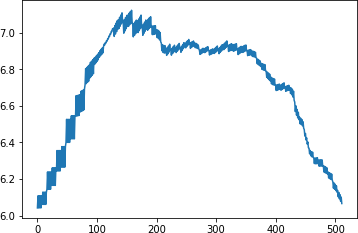
\includegraphics[width=0.5\linewidth]{15_4}
    \caption{График стандартных отклонений строк}
\end{figure}

В данном случае максимальной дисперсией обладает строка $i=158$, описывающая прямые с наклоном $\theta_{158} = \arctan\left( \frac{511}{158} \right) \approx 73^{\circ}$.
\begin{figure}[!h]
    \centering
    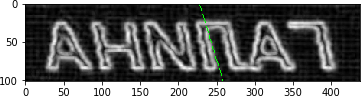
\includegraphics[width=0.5\linewidth]{15_5}
    \caption{Изображение со случайно выбранной прямой из найденного семейства}
\end{figure}

    \supersection{Способ использования БПХ для слепой компенсации радиальной дисторсии.}
        % Способ использования БПХ для слепой компенсации радиальной дисторсии.


    \supersection{Способ использования БПХ для определения степени сбития камеры. Эпиполярная геометрия.}
        % Способ использования БПХ для определения степени сбития камеры. Эпиполярная геометрия.


    \supersection{Быстрое вычисление суммы по любому отрезку и четырехвершиннику на изображении с помощью БПХ.}
        % Быстрое вычисление суммы по любому отрезку и четырехвершиннику на изображении с помощью БПХ.

Рассмотрим изображение размера $N \times N, N = 2^n$ в оттенках серого. Известно, что для любой пары пикселей существует по крайней мере одна содержащая их диадическая прямая. При этом все такие прямые приближают отрезок между ними одинаковым образом, поэтому задача вычисления суммы по отрезку, заданному двумя концами при помощи преобразования Хафа как минимум корректно поставлена. Для ее решения требуется научиться находить параметры какой-либо диадической прямой, проходящей через эту пару точек и вычислять сумму по любому отрезку известной прямой.

Для определенности будем рассматривать только преимущественно горизонтальные отрезки с положительным наклоном, то есть такие, что $y_2 \ge y_1, x_2 \ge x_1, \Delta y \le \Delta x$, где $(x_1, y_1)$ и $(x_2, y_2)$ -- координаты концов отрезка.

\paragraph{Определение диадического паттерна.}
Известно, что любой диадический паттерн $y = I_p(x), p \in \{ 0, 1, \dots, N-1\}$ может быть представлен в виде суммы некоторого подмножества множества $D = \left\{ I_1(x), I_2(x), I_4(x), \dots, I_N(x) \right\}$, где под суммой паттернов понимается паттерн, описываемый уравнением $y = I_{p_1}(x) + I_{p_2}(x)$. Отметим, что нам достаточно подобрать любой паттерн, удовлетворяющий условию $I_p\left( x_2 \right) - I_p\left( x_1 \right) = y_2 - y_1$. Для этого применим жадный алгоритм: выберем в качестве начального приближения горизонтальный паттерн $I_0(x)$ и на каждом шаге будем прибавлять самый <<большой>> паттерн из множества $D$, который не приводит к переполнению, то есть при котором $I_p\left( x_2 \right) - I_p\left( x_1 \right) \le y_2 - y_1$. Данный алгоритм всегда приводит к решению, следовательно, после $\Theta\left( \log N \right)$ операций мы получим параметр $t$, гарантирующий, что если паттерн проходит через первую точку, то он проходит и через вторую. Параметр $s$ подбирается очевидным способом так, чтобы паттерн действительно проходил через первую точку

\paragraph{Сумма по диадическому отрезку.}
Пусть задана диадическая прямая $y = s + I_t(x)$ и требуется вычислить сумму по всем точкам этой прямой на отрезке $0 \le x_1 \le x < x_2 \le N$.

Заметим, что для некоторых пар $(x_1, x_2)$ эта задача уже решается в процессе быстрого преобразования Хафа. А именно, на $k$-й итерации алгоритма в соответствующем массиве сохраняются такие суммы для всех $x_1 = m \cdot 2^k, x_2 = (m+1) \cdot 2^k$ по всем прямым. Несложно модифицировать алгоритм так, чтобы эти суммы были доступны после окончания вычислений, а не перезаписывались, для чего достаточно использовать для вычислений трехмерный массив. Это приведет к увеличению требований по памяти до $\Theta\left( N^2 \log N \right)$. При помощи этих значений сумма по любому отрезку с $x_1 = 0$ может быть вычислена при помощи жадного алгоритма, похожего на использованный в предыдущем пункте. Для произвольных значений $(x_1, x_2)$ следует вычислить сумму по двум отрезкам и взять разность. Итоговая сложность алгоритма составляет $\Theta\left( N^2 \log N \right)$ операций на предподсчет (БПХ), после чего сумма по каждому отрезку вычисляется за $O\left( \log N \right)$ операций.


Рассмотрим, как эта же методика может быть применена для вычисления сумм по произвольному выпуклому четырехвершиннику. Для этого применим к каждому столбцу кумулятивное суммирование так, чтобы каждый пиксель хранил сумму всех пикселей исходного изображения, расположенных в том же столбце не выше, чем он сам. Это преобразование выполняется линейным проходом по каждому столбцу за $\Theta\left( N^2 \right)$ операций. После такого преобразования сумма по произвольному отрезку фактически является суммой значений в исходном изображении по прямоугольной трапеции, одна из сторон которой обязательно находится на нижней строке изображения. Любой выпуклый четырехвершинник может быть представлен в виде суммы или разности не более чем четырех таких трапеций, следовательно, задача сводится к предыдущей и обладает такой же асимптотической сложностью: $\Theta\left( N^2 + N^2 \log N \right) = \Theta\left( N^2 \log N \right)$ операций на предподсчет и $O\left( 4 \log N \right) = O\left( \log N \right)$ операций на вычисление суммы по четырехвершиннику.

    \supersection{Сочетание БПХ и принципа четырех русских для случаях прямых в трехмерном пространстве.}
        % Сочетание БПХ и принципа четырех русских для случаях прямых в трехмерном пространстве.


    \supersection{Быстрая линейная бинарная кластеризация с помощью БПХ.}
        % Быстрая линейная бинарная кластеризация с помощью БПХ.


    \supersection{Робастное решение задачи линейной регресси путем вычисления M-оценок с помощью БПХ.}
        % Робастное решение задачи линейной регресси путем вычисления M-оценок с помощью БПХ.


\end{document}
